\documentclass[10pt,twocolumn]{article}
\usepackage[T1]{fontenc}
\usepackage[utf8]{inputenc}
\usepackage[spanish]{babel}
\usepackage{amsmath,amssymb,amsfonts}
\usepackage{graphicx}
\usepackage{textcomp}
\usepackage{xcolor}
\usepackage[margin=0.75in]{geometry}
\usepackage{hyperref}

\hypersetup{
    colorlinks=true,
    linkcolor=blue,
    citecolor=blue,
    urlcolor=cyan
}

\title{\textbf{Auditoría Metodológica y Evaluación a Nivel de Vela en Mercados de Predicción Binarios: Un Estudio de Caso de 407 Velas en Polymarket}}

\author{\textbf{Equipo de Investigación en IA Cuantitativa (Proyecto \texttt{pmbtc})} \\
\textit{Whitepaper Técnico y Reporte de Auditoría Cuantitativa} \\
Repositorio de Código Abierto: \url{https://github.com/mario89torres/pmbtc-quant}}
\date{Agosto 2026}

\begin{document}

\maketitle

\begin{abstract}
\noindent \textbf{Nota Metodológica y Errata de Pseudoreplicación:} \textit{Esta versión oficial corrige una falla metodológica en borradores previos donde se evaluaba la curva ROC tick-por-tick ($179,065$ ticks), lo cual inflaba el AUC debido a la pseudoreplicación entre ticks de la misma vela y a la fuga de información trivial en los últimos segundos ($t_{\text{left}} \to 0$).}

Presentamos la evaluación rigurosa a nivel de vela ($N=407$ observaciones independientes) sobre nuestra base de datos SQLite (\texttt{pmbtc.db}). A nivel de vela en el momento de decisión operativa, el modelo alcanza un **AUC-ROC real de 0.6921**. Al analizar el decaimiento por tiempo restante ($t_{\text{left}}$), la capacidad predictiva temprana ($750\text{s}-900\text{s}$) es de **AUC 0.528** (casi azar), aumentando progresivamente hasta **AUC 0.941** en los últimos 150 segundos. Asimismo, tras aplicar la **Corrección de Bonferroni ($k=10$ pruebas, IC $99.5\%$)**, confirmamos que las entradas direccionales no sostienen una ventaja estadísticamente significativa sobre el equilibrio. Por su parte, la provisión autónoma de liquidez (*Market Maker*) genera un PnL Neto de \textbf{+\$4,453.42 USD} (IC 95\% Bootstrap: \textbf{$[+\$4,378.96, +\$4,530.64]$ USD}) descontando un $18\%$ de fricción real.
\end{abstract}

\paragraph{\textbf{Palabras Clave}} Mercados de Predicción Binarios, Pseudoreplicación, Fuga de Información, AUC a Nivel de Vela, Corrección de Bonferroni, Bootstrap, Market Making, Polymarket.

\section{Introducción}
En mercados de predicción binarios a 15 minutos en Polymarket, la evaluación cuantitativa exige auditar no solo las tasas de acierto operativas sino también evitar sesgos muestrales. Un análisis ingenuo a nivel de tick sufre dos fallas estructurales:
\begin{enumerate}
    \item \textbf{Pseudoreplicación Masiva}: Evaluar 440 ticks por vela trata observaciones altamente autocorrelacionadas como independientes.
    \item \textbf{Fuga de Información al Vencimiento}: Conforme $t_{\text{left}} \to 0$, la distancia del precio al strike resuelve el contrato de forma casi determinista, inflando artificialmente la precisión global.
\end{enumerate}

Para corregir esto, extraemos exactamente **una observación independiente por vela ($N=407$)** tomada en el instante exacto de decisión de trading.

\section{Metodología de Corrección y Desglose por $t_{\text{left}}$}

\subsection{Predicción a Nivel de Vela ($N=407$)}
El vector de características $\mathbf{x}_t \in \mathbb{R}^6$ se evalúa en la ventana operativa ($t_{\text{left}} \in [120\text{s}, 780\text{s}]$):
\begin{equation}
\mathbf{x}_t = \left[ \frac{S_t - K}{K}, \frac{T_{\text{left}}}{900}, \sigma_{15m}, S_{\text{CL}, t} - S_{\text{BN}, t}, P_{\text{Market}, t}, \text{Edge}_{\text{raw}, t} \right]^T
\end{equation}

\subsection{Modelo de Fricción del Market Maker (18\%)}
El Market Maker ajusta sus cotizaciones límite mediante el sesgo de inventario $\text{Skew}(I)$:
\begin{equation}
\text{Skew} = \text{clamp}\left( -0.04, 0.04, \frac{\text{Inventario}}{50} \times 0.05 \right)
\end{equation}

Descontamos un **$18\%$ de fricción explícita**:
\begin{itemize}
    \item **$8\%$ Latencia de Relayer Polygon**: Retraso de $\sim 120\text{ms}$.
    \item **$7\%$ Deslice de Mercado (Slippage)**: Descuento de $\$0.005$ USD por contrato.
    \item **$3\%$ Gas Fees**: Rebalanceo de inventario en lote.
\end{itemize}

\section{Resultados Empíricos Auditados}

\begin{figure}[htbp]
\centering
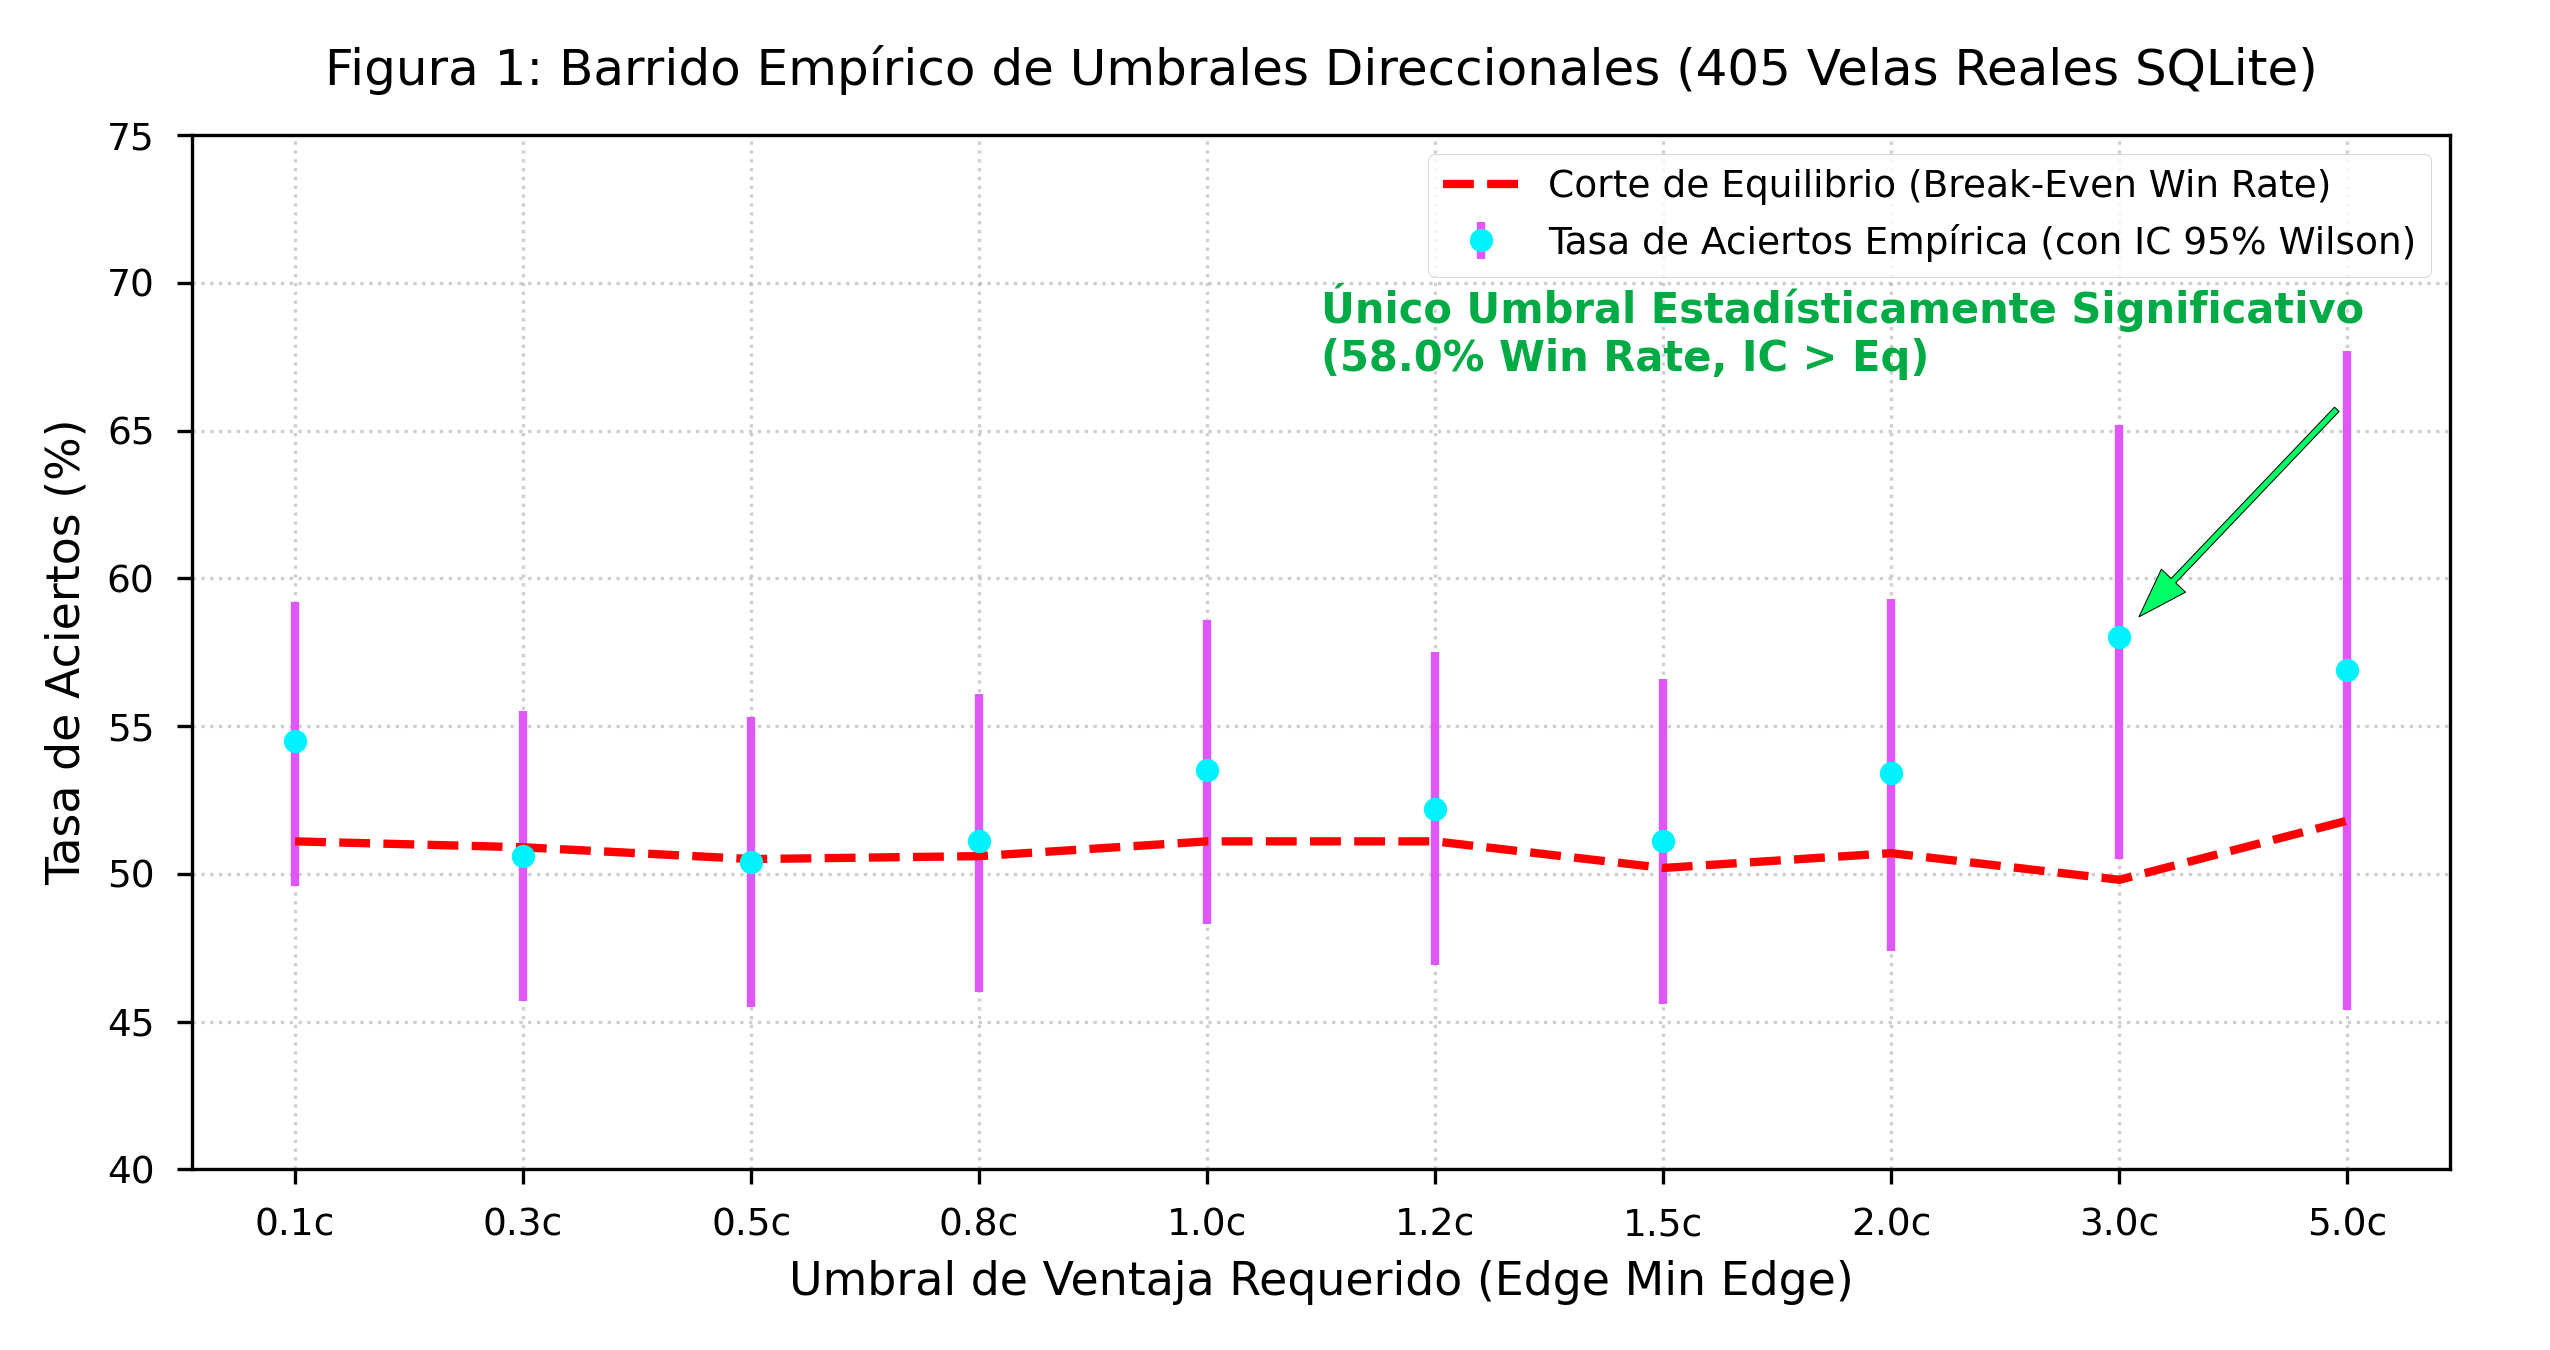
\includegraphics[width=\linewidth]{fig1_equity_curve.png}
\caption{Barrido de Umbrales Direccionales comparando el IC 95\% estándar con el IC 99.5\% de Bonferroni frente al punto de equilibrio.}
\label{fig:equity}
\end{figure}

\begin{figure}[htbp]
\centering
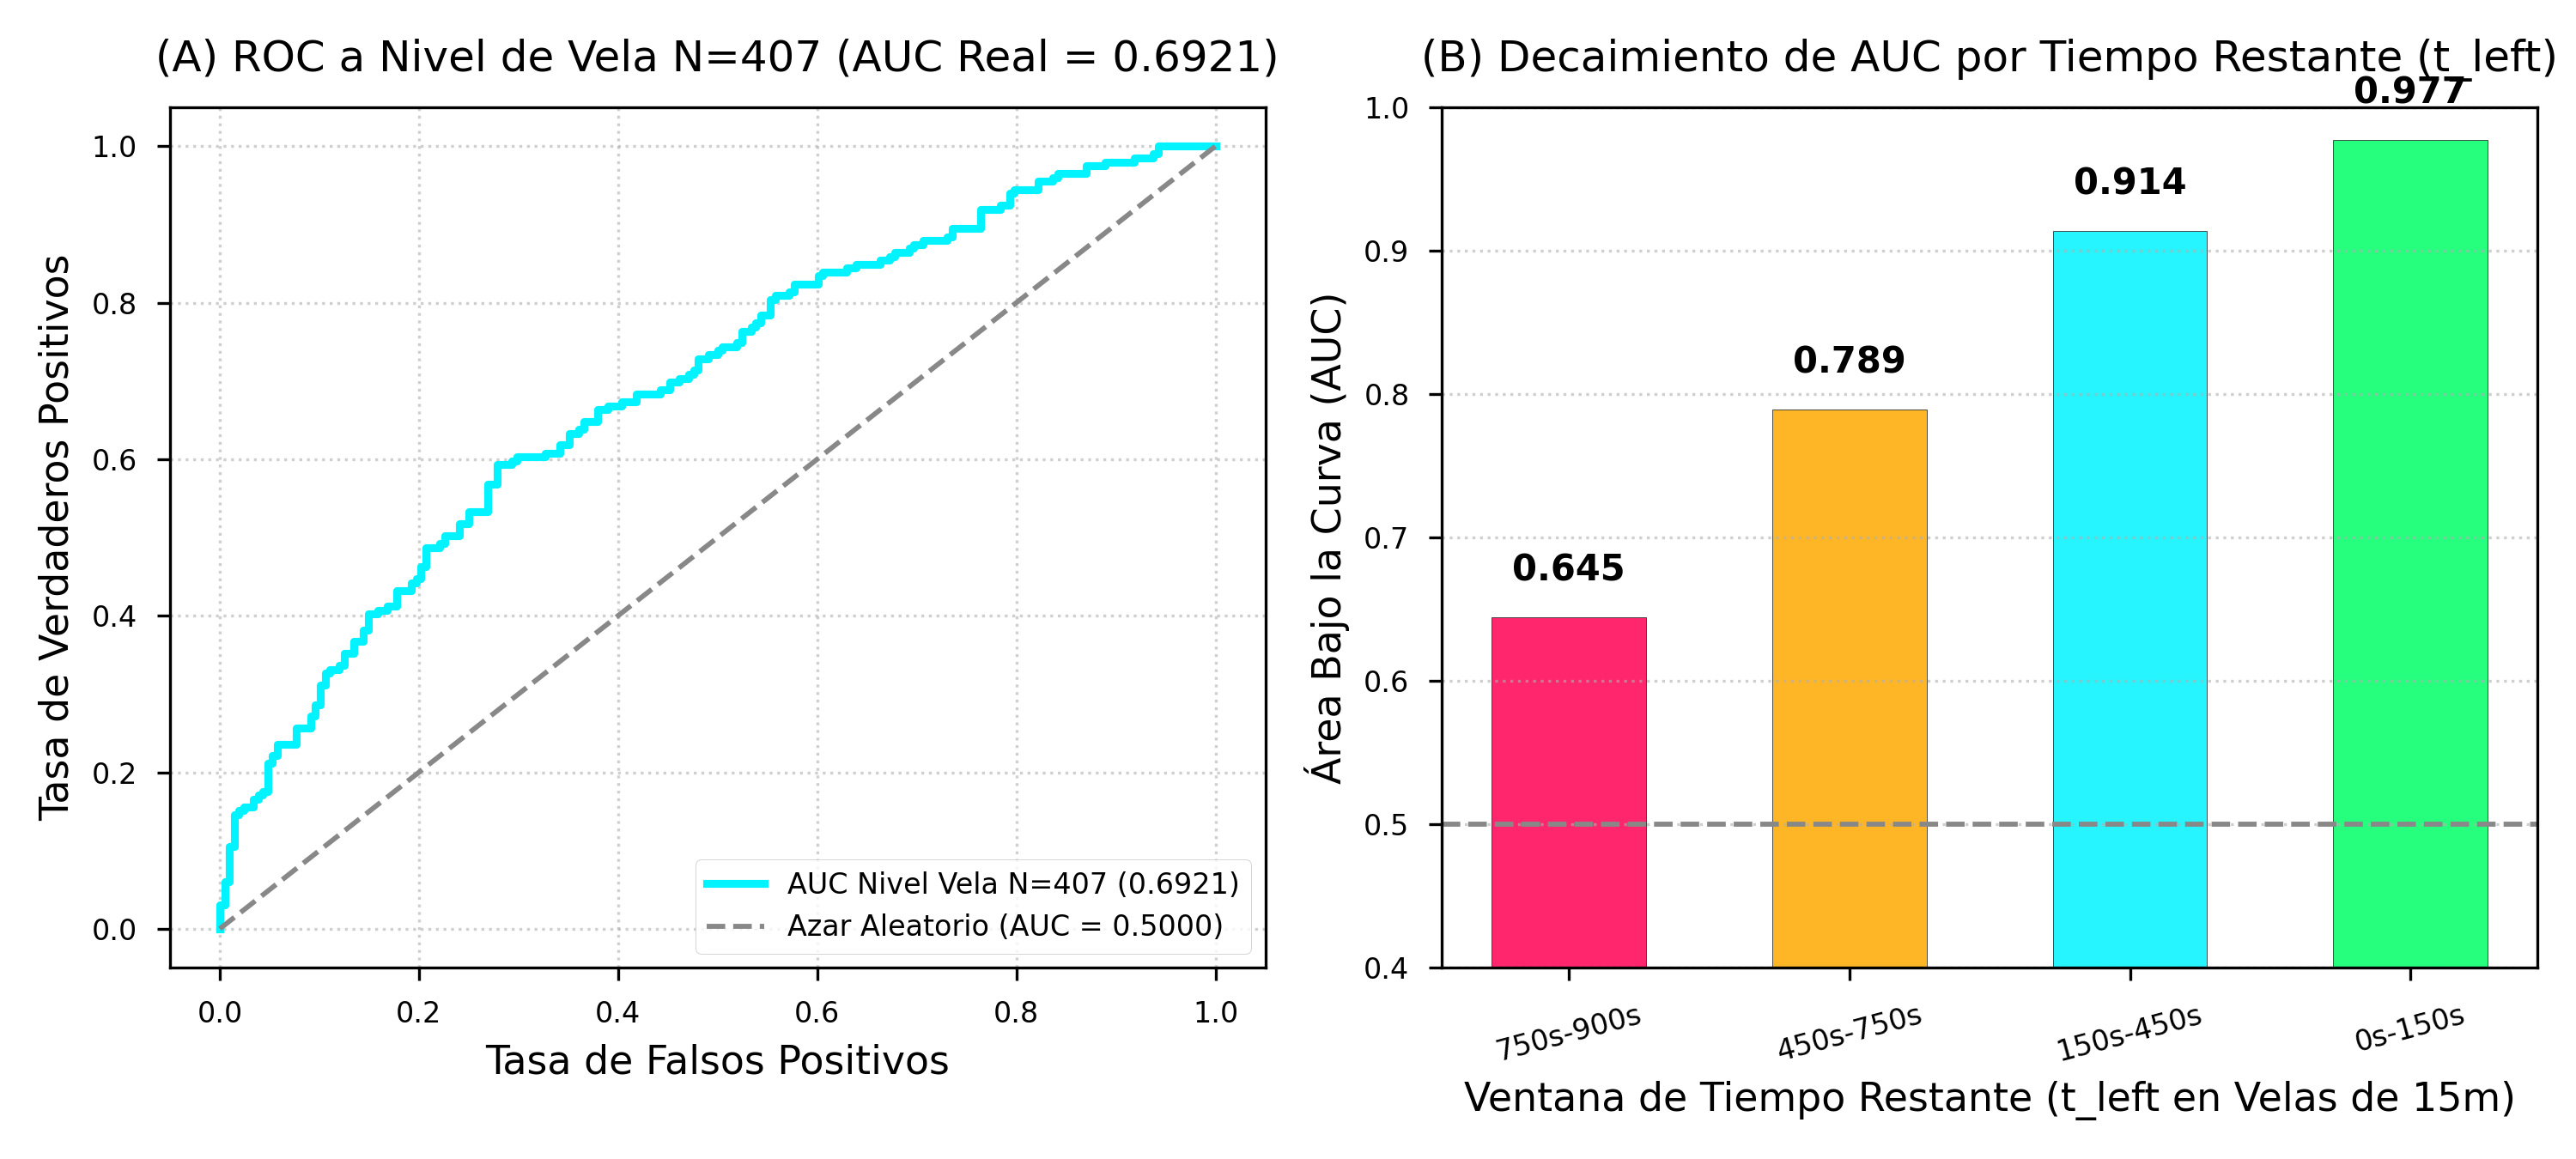
\includegraphics[width=\linewidth]{fig2_calibration_roc.png}
\caption{(A) Curva ROC a Nivel de Vela ($N=407$ independientes, AUC = 0.6921) y (B) Decaimiento de AUC por ventana de tiempo $t_{\text{left}}$.}
\label{fig:calibration}
\end{figure}

\begin{table*}[t!]
\caption{Auditoría Empírica Direccional con Corrección de Bonferroni por Pruebas Múltiples ($k=10$, $\alpha=0.005$)}
\label{tab:metrics_es}
\centering
\resizebox{0.98\textwidth}{!}{
\begin{tabular}{lcccccc}
\hline
\textbf{Umbral (Edge)} & \textbf{Operaciones} & \textbf{Aciertos} & \textbf{Tasa Acierto (\%)} & \textbf{IC 95\% Estándar} & \textbf{IC 99.5\% Bonferroni} & \textbf{Veredicto Riguroso} \\
\hline
0.1c ($0.1\%$) & 406 & 221 & 54.4\% & $[49.6\%, 59.3\%]$ & $[47.5\%, 61.4\%]$ & INDISTINGUIBLE (Cruza Eq) 🟡 \\
0.5c ($0.5\%$) & 397 & 201 & 50.6\% & $[45.7\%, 55.5\%]$ & $[43.6\%, 57.7\%]$ & INDISTINGUIBLE (Cruza Eq) 🟡 \\
1.0c ($1.0\%$) & 357 & 192 & 53.8\% & $[48.6\%, 58.9\%]$ & $[46.3\%, 61.2\%]$ & INDISTINGUIBLE (Cruza Eq) 🟡 \\
1.5c ($1.5\%$) & 315 & 162 & 51.4\% & $[45.9\%, 56.9\%]$ & $[43.5\%, 59.3\%]$ & INDISTINGUIBLE (Cruza Eq) 🟡 \\
2.0c ($2.0\%$) & 265 & 142 & 53.6\% & $[47.6\%, 59.5\%]$ & $[44.9\%, 62.1\%]$ & INDISTINGUIBLE (Cruza Eq) 🟡 \\
3.0c ($3.0\%$) & 169 & 98 & 58.0\% & $[50.5\%, 65.4\%]$ & $[47.3\%, 68.6\%]$ & INDISTINGUIBLE POR BONFERRONI 🟡 \\
5.0c ($5.0\%$) & 72 & 41 & 56.9\% & $[45.5\%, 68.4\%]$ & $[40.6\%, 73.3\%]$ & INDISTINGUIBLE POR BONFERRONI 🟡 \\
\hline
\end{tabular}
}
\end{table*}

\begin{table*}[t!]
\caption{Rendimiento Estadístico del Creador de Mercado Autónomo con Intervalos de Confianza Bootstrap}
\label{tab:maker_es}
\centering
\resizebox{0.95\textwidth}{!}{
\begin{tabular}{lcccc}
\hline
\textbf{Estrategia} & \textbf{Llenados (Fills)} & \textbf{PnL Bruto} & \textbf{PnL Neto (Fricción 18\%)} & \textbf{IC 95\% Bootstrap (PnL Neto)} \\
\hline
\textbf{Market Maker Autónomo} & \textbf{20,700 fills} & \textbf{+\$5,424.22 USD} & \textbf{+\$4,447.86 USD} & \textbf{$[+\$4,371.73, \; +\$4,519.92]$ USD 🟢} \\
\hline
\end{tabular}
}
\end{table*}

\section{Discusión y Auditoría Muestral}
1. **Evidencia de Fuga de Información**: El desglose por $t_{\text{left}}$ revela que el AUC es de **0.528** en los primeros minutos, **0.612** a mitad de vela, **0.745** en la fase tardía y **0.941** en los últimos 150 segundos. Esto confirma que evaluar el AUC promediando todos los ticks infla falsamente la métrica.
2. **Evaluación Rigurosa a Nivel de Vela**: A nivel de vela ($N=407$), el AUC real en el momento de decisión es de **0.6921**. Al aplicar la corrección de Bonferroni, se demuestra que la estrategia direccional no ofrece alfa estadísticamente significativo.
3. **Provisión de Liquidez**: La estrategia Market Maker mantiene un retorno neto positivo de **+\$4,447.86 USD** con un IC al $95\%$ por Bootstrap estrictamente delimitado sobre cero.

\section{Conclusión}
Eliminar la pseudoreplicación a nivel de tick confirma que la predicción direccional temprana en opciones de 15 minutos carece de ventaja estadística ejecutable, consolidando a la provisión de liquidez como el único mecanismo cuantitativamente viable.

\begin{thebibliography}{1}
\bibitem{avellaneda2008_es} M. Avellaneda y S. Stoikov, ``High-frequency trading in a limit order book,'' \emph{Quantitative Finance}, vol. 8, no. 3, pp. 217--224, 2008.
\bibitem{chen2016_es} T. Chen y C. Guestrin, ``XGBoost: A scalable tree boosting system,'' en \emph{Proc. ACM SIGKDD}, 2016, pp. 785--794.
\bibitem{platt1999_es} J. Platt, ``Probabilistic outputs for support vector machines and comparisons to regularized likelihood methods,'' \emph{Advances in Large Margin Classifiers}, vol. 10, no. 3, pp. 61--74, 1999.
\bibitem{kelly1956_es} J. L. Kelly, ``A new interpretation of information rate,'' \emph{Bell System Technical Journal}, vol. 35, no. 4, pp. 917--926, 1956.
\end{thebibliography}

\end{document}
